\subsubsection{Valensbånd}
Etter Niels Bohrr atommodell ligger elektroner i skall rundt atomkjernen.
\\
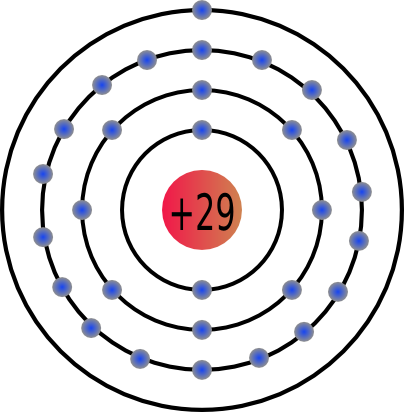
\includegraphics[width=0.25\textwidth]{./img/bohr-Cu}
\\
Kobberatom med 29 protoner og 29 elektroner.\\
Skall 1: 2 elektroner \\
Skall 2: 8 elektroner \\
Skall 3: 18 elektroner \\
Skall 4: 1 elektron
\\\\
Det ytterste elektronet har en svakere binding til kjernen og gjør at kobber leder strøm så godt.

\paragraph{Energigap} \mbox{} \\
Når man ser på de forskjellige energinivåene til disse skallene,
kalles de for bånd.
Det ytterste av disse båndene heter valensbåndet,
og hvis et elektron her blir eksitert vil det komme opp i ledningsbåndet.
I ledningsbåndet kan elektronet "flyte vekk" fra atomet.
\\
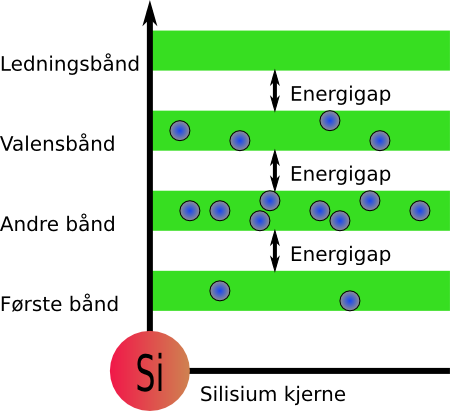
\includegraphics[width=0.5\textwidth]{./img/valence-Cu}



\subsubsection{Ledningsevne}
Energi-gapet mellom valensbåndet og ledningsbåndet
kan variere for forksjellige stoffer.
Store gap, som gjør det vanskelig for et elektron å nå ledningsbåndet,
er karakteristisk for isolatorer.
Tilsvarende er gapet mindre i halvledere.
Og i ledere er det er overlapp mellom valensbåndet og ledningsbåndet,
som gjør at det leder strøm ved romtemperatur.
\\\\
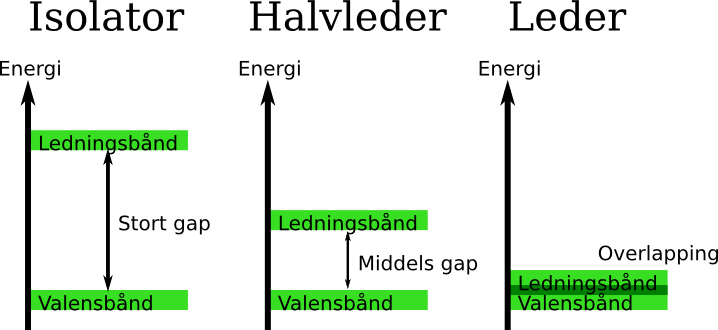
\includegraphics[width=\textwidth]{./img/energigap}




\subsubsection{Eksitasjon}
TODO

